\documentclass[twocolumn]{article}
\pdfoutput=1

% Roman numbers for sections
\renewcommand{\thesection}{\Roman{section}} 
\renewcommand{\thesubsection}{\thesection.\Roman{subsection}}

\usepackage{arxiv}

\usepackage[utf8]{inputenc} % allow utf-8 input
\usepackage[T1]{fontenc}    % use 8-bit T1 fonts
\usepackage{hyperref}       % hyperlinks
\usepackage{url}            % simple URL typesetting
\usepackage{booktabs}       % professional-quality tables
\usepackage{amsmath}
\usepackage{amsthm}
\usepackage{enumitem}
\setlist[itemize]{align=parleft,left=0pt..1em}
\setlist[enumerate]{align=parleft,left=0pt..1em}
\usepackage[font=scriptsize]{caption}
\usepackage{amsfonts}       % blackboard math symbols
\usepackage{nicefrac}       % compact symbols for 1/2, etc.
\usepackage{microtype}      % microtypography
\usepackage{lipsum}		% Can be removed after putting your text content
\usepackage{graphicx}
\usepackage{natbib}
\usepackage{doi}
\usepackage{listings,xcolor}

\lstdefinestyle{lua}{
  language=[5.3]Lua,
  basicstyle=\ttfamily,
  keywordstyle=\color{magenta},
  stringstyle=\color{blue},
  commentstyle=\color{black!50}
}

\title{Multidarkroom}

%\date{September 9, 1985}	% Here you can change the date presented in the paper title
%\date{} 					% Or removing it

\author{
    Denis Roio \\
	Dyne.org foundation \\
	Amsterdam, 1013AK \\
	\texttt{J@Dyne.org} \\
    \And
	Alberto Ibrisevic \\
	Laboratory of Cryptography\\
	Trento University (stage)\\
	\texttt{bettowski@dyne.org} \\
    \And
    Andrea D'Intino \\
    Dyne.org foundation \\
    Amsterdam, 1013AK \\
    \texttt{Andrea@Dyne.org} \\
}

% Uncomment to remove the date
%\date{}

% Uncomment to override  the `A preprint' in the header
\renewcommand{\headeright}{Dyne.org}
\renewcommand{\undertitle}{Zero Knowledge Multi Party Signatures with
  Application to Distributed Ledgers}
\renewcommand{\shorttitle}{\textit{Multidarkroom}}

\hypersetup{
  pdftitle={Multidarkroom - Zero-knowledge proof secured BLS multi-signatures},
  pdfsubject={cs.CR},
  pdfauthor={Denis Roio, Alberto Ibrisevic, Andrea D'Intino},
  pdfkeywords={Cryptography, signatures, zero-knowledge, multi-party, BLS, Coconut},
}

\begin{document}

\twocolumn[
  \begin{@twocolumnfalse}

\maketitle

\begin{abstract}
  Multidarkroom is a novel signature scheme supporting unlinkable
  signatures by multiple parties authenticated by means of a
  zero-knowledge credential scheme. Multidarkroom integrates with
  blockchains to ensure condidentiality, authenticity and availability
  even when credential issuing authorities are offline. We implement
  and evaluate a Multidarkroom smart contract for Zenroom and present
  an application related to multiple anonymous signatures by
  authenticated parties. Multidarkroom uses short and computationally
  efficient signatures and credentials whose verification takes the
  longest time to compute.
\end{abstract}

\vspace{2cm}

 \end{@twocolumnfalse}
]



\section{Introduction}

Multi-party computation [] applied to the signing process [] allows
the issuance of signatures without requiring any of the participating
parties to disclose secret signing keys to each other, nor requires
the presence of a trusted third-party to receive them and compose the
signatures. However, established schemes have shortcomings. Existing
protocols do not provide the necessary efficiency, re-randomization or
blind issuance properties necessary for the application to trustless
distributed systems. Those managing to implement such privacy
preserving features are prone to rogue-key attacks \citep{ietf-bls}
since they cannot grant that signatures are produced by legitimate key
holders.

The lack of efficient and privacy-preserving signature schemes impacts
distributed ledger platforms that support 'smart contracts' as well
distributed computing architectures where trust is not shared among
participants, but granted by one or more authorities through
credential issuance for the generation of non-interactive and
unlinkable proofs.

Multidarkroom uses short and computationally efficient signatures
composed of exactly two group elements that are linked to each
other. The size of the signature remains constant regardless of the
number of parties that are signing, while the credential size grows
linearly. Furthermure, after a one-time setup phase where the users
collect and aggregate a threshold number of verification keys from the
autorities, the attribute showing and verification O(1) in terms of
both cryptographic computations and communication of cryptographic
material, irrespective of the number of authorities.

Our evaluation of the Multiparty primities shows very promising
results. Verification takes about 10ms, while signing a document is
about 3 times faster.

\textbf{Contributions:} This paper makes three key contributions:

\begin{itemize}

\item We describe the signature scheme underlying Multidarkroom,
  including how key generation, signing and verification operate
  (Section \ref{sec:signature}). The scheme is an application of the
  BLS signature scheme \citep{asiacrypt-bls} fitted with features to
  grant the unlinkability of signatures and to secure it against
  rogue-key attacks.

\item We describe the credential scheme underlying Multidarkroom,
  including how key generation, issuance, aggregation and verification
  of credentials operate (Section \ref{sec:credential}). The scheme is
  an application of the Coconut credential scheme \citep{coconut-2018}
  that is general purpose and can be scaled to a fully distributed
  threshold issuance that is re-randomizable.

\item We implement a Zencode scenario of Multidarkroom to be executed
  on and off-chain by the Zenroom VM, complete with functions for
  public credential issuance, signature session creation and
  multi-party non-interactive signing (Section
  \ref{sec:implementation}). We evaluate the performance and cost of
  this implementation on on-site and on-line platforms leveraging
  end-to-end encryption (Section \ref{sec:evaluation}).

\end{itemize}

% I. Signature scheme (BLS)
\section{Signature}
\label{sec:signature}

Throughout this and the next section we will adopt the following notations: 
\begin{itemize}
    \item $\mathbb{F}_p$ is the prime finite field with $p$ elements (i.e. of prime order $p$). In our case the prime is long 383 bits;
    \item $E$ denotes the (additive) group of points of the curve BLS-383 of order $n$ which can be described with the Weierstrass form  $y^2=x^3 + 16$; 
    \item $E_T$ represents instead the group of points of the twisted curve of BLS-383, with embedding degree $k=12$. The order of this group is also $n$;
\end{itemize}
We also require defining the notion of a cryptographic pairing. Basically it is a function $e: \mathbb{G}_1\times\mathbb{G}_2\to \mathbb{G}_T$, where $\mathbb{G}_1,\mathbb{G}_2$ and $\mathbb{G}_T$ are all groups of same order $n$, such that satisfies the following properties:
\begin{itemize}
    \item [i.] \emph{Bilinearity}, i.e. given $P,Q\in\mathbb{G}_1$ and $R,S\in\mathbb{G}_2$, we have 
    \begin{align*}
        e(P+Q,R) = e(P,R)\cdot e(Q,R) \\
        e(P,R+S) = e(P,R)\cdot e(P,S)
    \end{align*}
    \item[ii.] \emph{Non-degeneracy}, meaning that for all $g_1\in\mathbb{G}_1, g_2\in\mathbb{G}_2$, $e(g_1,g_2)\ne 1_{\mathbb{G}_T}$, the identity element of the group $\mathbb{G}_T$;
    \item[iii.] \emph{ Efficiency}, so that the map $e$ is easy to compute;
    \item[iv. ] $\mathbb{G}_1\ne \mathbb{G}_2$, and moreover, that there exist no efficient homomorphism between $\mathbb{G}_1$ and $\mathbb{G}_2$.
\end{itemize}
For the purpose of our protocol we will have $\mathbb{G}_1 = E_T$ and $\mathbb{G}_1 = E$, and $\mathbb{G}_T\subset \mathbb{F}_{p^{12}}$ is the subgroup containing the $n$-th roots of unity. Instead $e: E_T  \times E\to \mathbb{G}_T$ is the \emph{Miller pairing}, which in our code is referred as the method \verb!miller(ECP2 P, ECP Q)!. \\
A \emph{BLS signature} is a signature scheme whose design exploits a cryptographic pairing. As for other well known algorithm such as ECDSA, it will work following these four main steps:
\begin{itemize}
    \item  \textbf{Key Generation phase.} For a user who wants to sign a message $m$, a secret key $sk$ is randomically chosen uniformly in $\mathbb{F}_n$, where $n$ is the order of the groups $\mathbb{G}_1, \mathbb{G}_2, \mathbb{G}_T$. The corresponding public key $pk$ is the element $sk\cdot G_2\in E_T$;
    \item \textbf{Session Generation.} Anyone willing to start a signing session on a message $m$ will create:
    \begin{itemize}
       \item[1.] a random $r$ and its corresponding point $R = r\cdot G_2$
       \item[2.] the sum of $R$ and all $pk$ supposed to participate to the signature such as $P = R + \sum_i pk_i$
       \item[3.] the unique identifier of the session calculated as hash to point of the message $m$, such as $UID = H(m)\in E$
       \item[4.] the first layer of the signature $S \leftarrow r\cdot UID$, later to be summed with all other signatures in a multi-party computation setup resulting in the final signature as $S \leftarrow r\cdot UID + \sum_i sk_i\cdot UID$
       \item[5.] the array of unique fingerprints of each signature resulting from the credential authentication (see section \ref{credential}) such as $\{\zeta_{i_1},\dots,\zeta_{i_n}\}$
    \end{itemize}
    \item   \textbf{Signing phase.} The message $m$ is first hashed into a point $H\in E$ using a cryptographic hash function (treated as a random oracle), which in our scheme is done by the method \verb!hashtopoint!; the related signature is then given by $\sigma = sk\cdot P$;
    \item   \textbf{Verification phase.} For an other user that wants to verify the authenticity and the integrity of the message $m$, it needs to
    \begin{itemize}
        \item [1.] parse $m, pk$ and $\sigma$
        \item [2.] hash the message $m$ into the point $H$ and then check if the following identity holds,
        \[
        e(pk,H) = e(G_2,\sigma)
        \]
    \end{itemize}
\end{itemize}
If verification passes it means that $\sigma$ is a valid signature for $m$ and the protocol ends without errors.
\begin{proof}
 [Proof of the verification algorithm:] By using the definitions of the elements involved and exploiting the property of the pairing $e$ we have
\[
\begin{split}
    e(pk,H) &= e(sk\cdot G_2, H) \\
            &= e(G_2,H)^{sk}\\
            &= e(G_2,sk\cdot H)\\
            &= e(G_2,\sigma)
\end{split}
\]
\end{proof}
BLS signatures present some interesting features. For instance, the length of the output $\sigma$ competes to those obtained by ECDSA and similar algorithms; in our specific case, by using BLS-383, it will be 32 Bytes long, which is typically a standard nowadays. Then, since this curve is also pairing-friendly, with the assumption made on $e$, the signature is produced in a very short time. Moreover, BLS supports also aggregation, that is the ability to aggregate a collection of multiple signatures $\sigma_i$ (each one related to a different message $m_i$) into a singular new object $\sigma$, that can be validated using the respective public keys $pk_i$. This is possible thanks to the fact that $\sigma_i\in G_1 \forall i$, giving to the algorithm an homomorphic property. We will show now how this last feature can be attained specifically for two signatures using the same message $m$ but different partecipants:
\begin{itemize}
    \item after collecting the signatures $\sigma_1$ and $\sigma_2$, to compute the new cryptographical object first of all we generate a base point $R= r\cdot H$, where $r\in\mathbb{F}_n$ is randomly generated and $H$ is again the hashed point derived from $m$;\\
    \item the aggrageted $\sigma$ is then obtained by simply summing $R+\sigma_1+\sigma_2$;
    \item in order to verify that $\sigma$ is valid we compute $P = pk_R + pk_1 + pk_2$, where $pk_R = r\cdot G_2$, that works as a public key with respect to the nonce $r$, which instead is kept secret. Verification is then performed by checking if the following identity holds
    \[ 
    e(P,H) = e(G_2,\sigma)
    \]
\end{itemize}
If verification passes without errors it means that $\sigma$ is a valid aggregated signature of $m$.
\begin{proof}
By recalling that $\sigma = R + \sigma_1 + \sigma_2$, $P = pk_R + pk_1 + pk_2$, by using the property of the pairing $e$ we have
\[
\begin{split}
    e(P,H)  &= e(pk_R + pk_1 + pk_2, H) \\
            &= e((r + sk_1 + sk_2)\cdot G_2,H)\\
            &= e(G_2,H)^{r + sk_1 + sk_2}\\
            &= e(G_2,(r + sk_1 + sk_2)\cdot H) \\
            &= e(G_2,R + \sigma_1 + \sigma_2) \\
            &= e(G_2,\sigma)
\end{split}
\]
\end{proof} 
We conclude this section with a final consideration on this feature. We recall that in the generation of the aggregated signature $\sigma$ we used as a starting point the variable $R = r\cdot G_2$, but in literature it is also common to find instead simply the base point $G_2$. The choice of randomizing it (providing that the random number generator acts as an oracle) helps in preventing replay attacks, since the signature generated by the process is linked to the session in which is produced, for if an attacker managed to get some information from $\sigma$, it would be difficult to use it in order to forge new signatures.
\section{Credential}
\label{sec:credential}

Following the guidelines of Coconut, the credentials issuing scheme works as follows:
\begin{itemize}
\item [1.] the issuer generates its own keypair $(s_k,v_k)$, where $s_k=(x,y)\in\mathbf{Z}^2$ is the pair of secret scalars (the signing key) and $v_k=(\alpha, \beta)=(x\cdot G_2,y\cdot G_2)$ is the verifying key, made by the related pair of public points over the twisted elliptic curve of BLS-383 of embedding degree $k=12$; 
\item [2.] the user $i$, with its respective keys $(sk_i, PK_i)$ make a credential request on its secret attribute $ck_i\in\mathbf{Z}$ to the issuer, sending $\lambda$ which contains a zero-knowledge proof $\pi_s$ of the authenticity of user $i$; 
\item[3.] the issuer, after having received $\lambda$, verifies the proof $\pi_s$ at its inside, and if it passes, then releases to user $i$ a credential $\tilde{\sigma}$ signed used its own key $sk$.
\end{itemize}
Step 1. is self-explanatory. Steps 2. and 3. require a bit more effort, in fact in order to build a valid request $\lambda$, and so also a valid proof $\pi_s$, first of all the user must produce an hash digest $H(ck_i)$ for the attribute $ck_i$, that we call $m$, then computes two more variables $c$ and $s$ defined as
\begin{align*}
c &= r\cdot G_1 + m\cdot HS \\
s_m &= (a,b) = (k \cdot G_1, k\cdot \gamma + m\cdot c)
\end{align*}
where $r$ and $k$ are fresh randomly generated integers, $G_1$ is the base point of the elliptic curve BLS-383, and $HS$ is an hard-encoded point of the same curve. These two variables are alleged in the credential request $\lambda$ produced in \verb!prepare_blind_sign! and are needed to the verifier to assure the authenticity of the user through the proof $\pi_s$, which requires as input $m, k, r, c$ and $ck_i\cdot G_1$ (called also $\gamma$). The Non-Iteractive Zero Knowlwdge proof (for short NIZK proof) $\pi_s$ generated by the function \verb!blind_sign! is computed as follows:
\begin{itemize}
    \item \textbf{Randomization phase.} Three new nonces $w_m, w_k, w_r\in \mathbf{Z}$ are generated, each one related to the input variables $m, k, r$ respectively as we will show soon; 
    \item \textbf{Challenge phase.} The protocol creates three commitment values, namely $A_w, B_w, C_w$ defined as follows
    \begin{align*}
        A_w &= w_k\cdot G_1 \\ 
        B_w &= w_k\cdot\gamma + w_m\cdot c \\
        C_w &= w_r\cdot G_1 + w_m \cdot HS
    \end{align*}
    Then these variables are used as input of a function $\varphi$ producing an integer $c_m=\varphi(\{c,A_w,B_w,C_w\})$;
    \item \textbf{Response phase.} In order that the proof can be verified the protocol generates three more variables which are alleged inside the proof itself and link the nonces $w_m, w_k, w_r$ with $m, k, r$, i.e:
    \begin{align*}
        r_m &= w_m - c_m m \\
        r_k &= w_k - c_m k \\
        r_r &= w_r - c_m r
    \end{align*}
\end{itemize}
So basically, the proof $\pi_s$ contains the three response variables $r_m, r_k, r_r$ and also the commitment value $c_m$, that can be used for a predicate $\phi$ which is true when computed on $m$. Once the verifier receives the request $\lambda$, in order to check if the proof is valid it should be able to reconstruct  $A_w, B_w, C_w$ by doing these computations,
\begin{align*}
\widehat{A}_w &= c_m\cdot a + r_k\cdot G_1 \\
\widehat{B}_w &= c_m\cdot b + r_k\cdot \gamma + r_m\cdot c \\
\widehat{C}_w &= c_m\cdot c + r_r\cdot G_1 + r_m\cdot HS
\end{align*}
If the request is correct, then we will have that 
\begin{equation}\label{challenge pi_s}
\varphi(\{c,\widehat{A}_w,\widehat{B}_w,\widehat{C}_w\}) = \varphi(\{c,A_w,B_w,C_w\}) = c_m
\end{equation}
and verification is thus complete, meaning that the verifier has right to believe that the prover actually owns the secret attribute $ck_i$ associated to the public variable $\gamma$ and that consequently has produced a valid commitment $c$ and (El-Gamal) encryption $s$; in other words,
\begin{align*}
\pi_s = \text{ NIZK}\{&(ck_i, m, r, k): \\
&\gamma = ck_i\cdot G_1, \\
&c = r\cdot G_1 + m\cdot HS, \\
&s_m = (k \cdot G_1, k\cdot \gamma + m\cdot c), \\
&\phi(m)=1\}
\end{align*}
At this point the user will now have a blind credential $\tilde{\sigma} = (c, \tilde{a}, \tilde{b})$ issued by the authority, where
\begin{align*} \\
\tilde{a} &= y \cdot a \\
\tilde{b} &= x\cdot c + y\cdot b
\end{align*}
 The user then will have to unblind it using its secret credential key, obtaining $\sigma = (c, s) = (c, \tilde{b} - ck_i (\tilde{a}))$, which will use to prove its identity when signing a message. The procedure is similar to the one seen before with some extra details:
\begin{itemize}
    \item \textbf{Setup.} As for the the BLS signature, an elliptic point $H$, associated to the hash of the message to sign, is required as an Unique Identifier (\verb!UID!) for the signing session;
    \item \textbf{Credential proving.} The user produces two cryptographical objects $\theta$ (containing a new proof $\pi_v$) and $\zeta$ (which is unequivocally associated to $H$) through \verb!prove_cred_uid!, taking as input its own credential $\sigma$, the related secret attribute $c_k$, the authority public key $v_k = (\alpha, \beta)$ and the session point $H$.
\end{itemize}
The new objects $\theta$ and $\zeta$ are derived as follows:
\begin{itemize}
    \item as before the user hashes $ck$ into $m$, and this time generates two random values $r$ and $r'$;\\
    \item next, it randomizes its credential $\sigma$ into $\sigma' = (c', s') = (r'\cdot c, r'\cdot s)$ and then computes two elliptic curve points $\kappa$ and $\nu$ as
    \begin{align*}
        \kappa &= \alpha + m\cdot\beta + r\cdot G_2\\
        \nu &= r \cdot c'
    \end{align*}\\
    \item finally, the resulting $\theta$ is the t-uple $(\kappa, \nu, \pi_v, \phi')$, where $\pi_v$ is a valid zero knowledge proof of the following form
    \begin{align*}
        \pi_v = \text{ NIZK}\{&(m, r): \\
        &\kappa = \alpha + m\cdot\beta + r\cdot G_2\\
        &\nu = r \cdot c' \\
        &\phi'(m)=1\}
    \end{align*}
    with $\phi'$ being a predicate which is true on $m$, while $\zeta$ is simply the scalar multiplication $m\cdot H$.
\end{itemize}
Building the proof $\pi_v$ requires similar steps as seen for $\pi_s$, in fact we create three commitment values $A_w, B_w, C_w$ defined as
\begin{align*}
    A_w &= \alpha + w_m\cdot \beta + w_r \cdot G_2 \\
    B_w &= w_r\cdot c' \\
    C_w &= w_m\cdot H
\end{align*}
where $w_m, w_r$ are fresh generated nonces; then we set the challenge as the computation of $c_m=\varphi(\{\alpha,\beta,A_w,B_w,C_w\})$ with the related responses 
\begin{align*}
    r_m &= w_m - mc \\
    r_r &= w_r - rc
\end{align*}
The values of $r_m$ and $r_r$ are stored inside $\pi_v$ which will be then sent through $\theta$ (together with $\zeta$) from the prover to the verifier. In order to check that the user has legitimately generated the proof and at the same time is the owner of the credential the following steps must be made:
\begin{itemize}
    \item[1.] extracting $\kappa, \nu, \pi_v$ (which is $(r_m,r_r, c_m))$ from $\theta$;
    \item[2.] reconstructing the commitments $A_w, B_w, C_w$ as
    \begin{align*}
        \widehat{A}_w &= c_m\cdot \kappa + r_r\cdot G_2 + (1 - c_m) \cdot\alpha + r_m \cdot \beta \\
        \widehat{B}_w &= r_r\cdot c' + c_m\cdot \nu \\
        \widehat{C}_w &= r_m\cdot H + c_m\cdot \zeta
    \end{align*}
    \item[3.] checking either that
    \begin{multline}\label{challenge pi_v}  \varphi(\{\alpha,\beta,\widehat{A}_w,\widehat{B}_w,\widehat{C}_w\}) = \\ \varphi(\{\alpha,\beta,A_w,B_w,C_w\}) = c_m,
    \end{multline}
    that $c' \ne O$, the point at infinity, and that
    \begin{equation}\label{miller}
    e(\kappa, c') = e(G_2, s' + \nu)
    \end{equation}
    where $e$ is the Miller pairing function defined as
    \[
    e: E_T \times E \to \mathbb{F}_{p^{12}}
    \]
    (\textbf{probabile che quest'ultima definizione la scrivero nella sezione 2})
\end{itemize}
Actually the predicate $\phi$ in the definition of $pi_v$ can be thought as performing steps 2. and 3. and, if any of these fails the protocol will abort returning a failure, otherwise verification passes and the user can finally produce the signature.\\
\paragraph{Proof of the verification algorithms.} We now show for the proof $\pi_s$ that actually by using the responses $r_m, r_k$ and $r_r$, together with $c_m$ and the other parameters inside $\lambda$, i.e. $s=(a,b), c$ and $\gamma$, using also the hard coded point $HS$, it is possible to reconstruct the commitments $A_w, B_w, C_w$:
\begin{align*}
    \widehat{A}_w   &= c_m\cdot a + r_k\cdot G_1 = c_m k \cdot G_1 + r_k \cdot G_1 \\
                    &= (c_m k + r_k)\cdot G_1 = (c_m k + w_k - c_m k)\cdot G_1 \\
                    &= w_k\cdot G_1 = A_w \\
    \widehat{B}_w   &= c_m\cdot b + r_k\cdot \gamma + r_m\cdot c \\
                    &= c_m\cdot (k\cdot \gamma + m\cdot c) + r_k\cdot\gamma + r_m\cdot c \\
                    &= (c_m k + r_k) \cdot\gamma + (c_m m + r_m\cdot c) \\
                    &= (c_m k + w_k - c_m k ) \cdot\gamma + (c_m m + w_m - c_m m)\cdot c) \\
                    &= w_k\cdot\gamma + w_m\cdot c = B_w \\
    \widehat{C}_w   &= c_m\cdot c + r_r\cdot G_1 + r_m\cdot HS \\
    &= c_m\cdot (r\cdot G_1 + m\cdot HS) + r_r\cdot G_1 + r_m\cdot HS \\
                    &= (c_m r + r_r) G_1 + (c_m m + r_m) HS \\
                    &= (c_m r + w_r - c_m r)\cdot G_1 + (c_m m + w_m - c_m m)\cdot HS \\
                    &= w_r \cdot G_1 + w_m\cdot HS = C_w
\end{align*} 
Regarding the second proof $\pi_v$, we have to prove both the identities (\ref{challenge pi_v}) and (\ref{miller}) hold. We will focus only on the latter since the former requires a similar approach on what we have have done for $\pi_s$, but with different parameters involved ($\kappa, \nu$, etc.). The LHS of the relation can be expressed as
\begin{align*}
    e(\kappa, c') &= e(\alpha + m\cdot\beta + r\cdot G_2, c') \\
    &= e(x\cdot G_2 + my\cdot G_2  + r\cdot G_2,\tilde{r}\cdot G_1) \\
    &= e((x+my+r)\cdot G_2, \tilde{r}\cdot G_1) \\
    &= e(G_2,G_1)^{(x+my+r)\tilde{r}}
\end{align*}
using the substitution $c'=\tilde{r}\cdot G_1$, with $\tilde{r}\in\mathbb{F}_p$ since we know that $c'\in E$. For the RHS we have instead
\begin{align*}
    e(G_2, s' + \nu) &= e(G_2, r'\cdot s + r \cdot c') \\
    &= e(G_2, r'(\tilde{b} - ck_iy (\tilde{a})) + r \cdot c') \\
    &= e(G_2, r'(x\cdot c + y\cdot b - ck_iy\cdot a) + r \cdot c') \\
    &= e(G_2, r'(x\cdot c + y\cdot b - ck_iy\cdot a + r \cdot c)) 
\end{align*}
The second argument of the pairing can be rewritten as
\[
\begin{split}
    &r'(x\cdot c + y\cdot b - ck_iy\cdot a + r \cdot c) = \\
    &r'(x\cdot c + y(k\cdot \gamma + m\cdot c) - ck_iyk\cdot G_1 +     r \cdot c) = \\
    &r'(x\cdot c + ym\cdot c +         ykck_i\cdot G_1  - ykck_i\cdot     G_1 + r \cdot c) = \\
    &r'(x + ym + r) \cdot c
\end{split}
\]
So, at the end
\[
\begin{split}
    e(G_2, s' + \nu) &= e(G_2, r'(x\cdot c + y\cdot b - dy\cdot a + r \cdot c)) \\
    &= e(G_2, r'(x + ym + r) \cdot c) \\
    &= e(G_2,(x+my+r)\tilde{r}\cdot G_1) \\
    &= e(G_2,G_1)^{(x+my+r)\tilde{r}}
\end{split}
\]
and (\ref{miller}) is finally proved. 
\qed

\paragraph{Security considerations.} 
As mentioned in \citep{coconut-2018}, BLS signature and the proof system obtained with Coconut are considered secure by assuming the the existence of random oracles, together with the decisional Diffie-Hellman Problem (DDH), the external Diffie-Hellman Problem (XDH), and with the Lysyanskaya-Rivest-Sahai-Wol Problem (LRSW), which are connected to the Discrete Logarithm. In fact, under these assumptions, we have that our protocol satisfies uforgeability, blindness, and unlinkability.

\section{Implementation}
\label{sec:implementation}

\lstset{basicstyle=\ttfamily\scriptsize, breaklines=true}

In this section we illustrate our implementation of Multidarkroom
keygen, sign and verify operations outlining for each:

\begin{enumerate}
  \item the communication sequence diagram (figure)
  \item the Zenroom code (Lua dialect script)
  \item the Zencode statements
\end{enumerate}

In addition to the above, a Setup operation will be briefly
illustrated without the sequence diagram, as it includes the local
creation of a keypair for the Issuer who will validate the
credentials.

\textbf{Setup:} Generate the Issuer keys for credential signature

\begin{lstlisting}[style=lua]
 x = INT.random()
 y = INT.random()
 sk = { x = x,
        y = y  }
 vk = { alpha = G2 * x,
        beta  = G2 * y  }
 return { sign = sk,
          verify = vk }
\end{lstlisting}

Executed by the Zencode utterance:

\textbf{When I create the issuer keypair}

It will create a new \emph{issuer keypair} that can be used to sign
each new \emph{credential request}. Its public member \emph{.verify}
should be public and know to anyone willing to verify the credentials
of signers.

\textbf{Keygen:} Generate a credential request and have it signed by
an Issuer, as well generate a BLS keypair used to sign documents. This
procedure will generate private keys that should not be comunicated,
as well public BLS keys that can be aggregated for signature
verification.

Figure~\ref{fig:keygen} illustrates how this process consists of two
different function calls: \verb!keygen! to create an ElGamal keypair
and \verb!prepare_blind_sign! to generate a Coconut credential
request. An interactive exchange takes place between the Signer and
the Issuer that verifies the possession of the secret ElGamal key and
signs a credential to witness this condition.

\begin{figure}
  \caption{Keygen process sequence diagram}
  \label{fig:keygen}
  \centering
  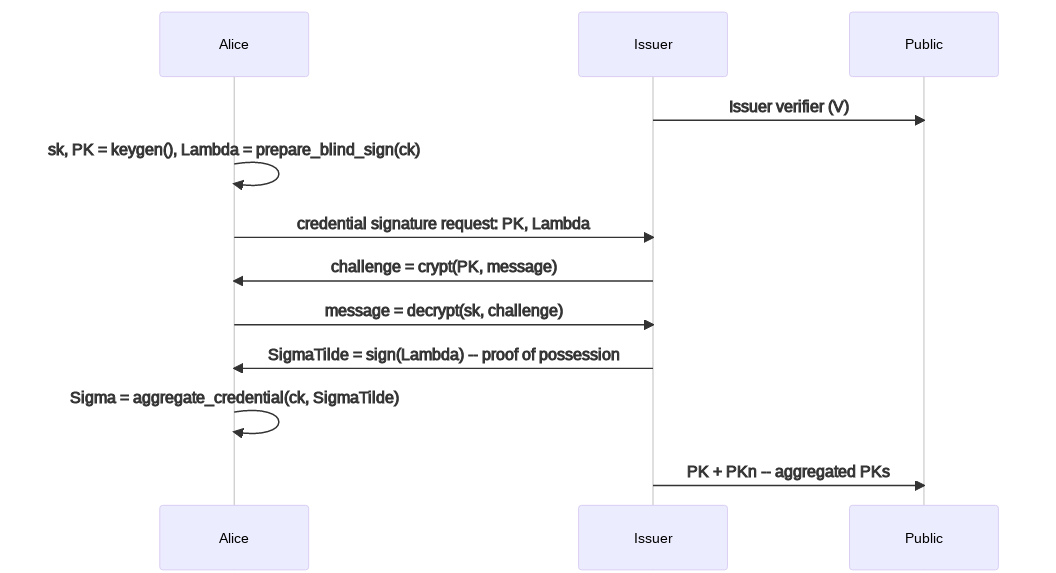
\includegraphics[width=0.5\textwidth]{keygen-seq}
\end{figure}

The public key of the Issuer which is used to sign the credential
should have been public and known by the Signer at the beginning of
the keygen process, while at the end of this process the public
ElGamal key should be published, i.e. on a distributed ledger.

The following Zenroom implementation makes use of the Coconut
built-in extension for zero-knowledge proof credentials.

\begin{lstlisting}[basicstyle=\tiny,style=lua]
ZK = require_once('crypto_abc')
issuer = ZK.issuer_keygen() -- setup
sk = INT.random() -- signing key
ck = INT.random() -- credential key
PK = G2 * sk     -- signature verifier
Lambda =
 ZK.prepare_blind_sign(ck * G1, ck)
SigmaTilde =
 ZK.blind_sign(issuer.sign, Lambda)
Sigma =
 ZK.aggregate_creds(ck, {SigmaTilde})
\end{lstlisting}

This code is executed in multiple steps by the Zencode utterances:

\begin{enumerate}

\item \textbf{When I create the credential keypair}

  will create a new \emph{credential keypair} object containing
  members \emph{public} (ECP) and \emph{private} (BIG).

\item \textbf{When I create the credential request}

  will use the \emph{credential keypair} to create a new
  \emph{credential request} complex schema object for ZK proof.

\item \textbf{When I create the credential signature}

  will be executed by the Issuer after the proof-of-possession
  challenge is positive (exchange and confirmation of an encrypted
  message using BLS public keys) to sign the credential.

\item \textbf{When I create the credentials}

  will aggregate one or more \emph{credential signature} (SigmaTilde)
  together with the \emph{private} member of the \emph{credential
    keypair} and finally create \emph{credentials} capable of
  producing Zero-Knowledge proofs of possession.

\end{enumerate}



\textbf{Sign:}

\begin{figure}
  \caption{Signing process sequence diagram}
  \centering
  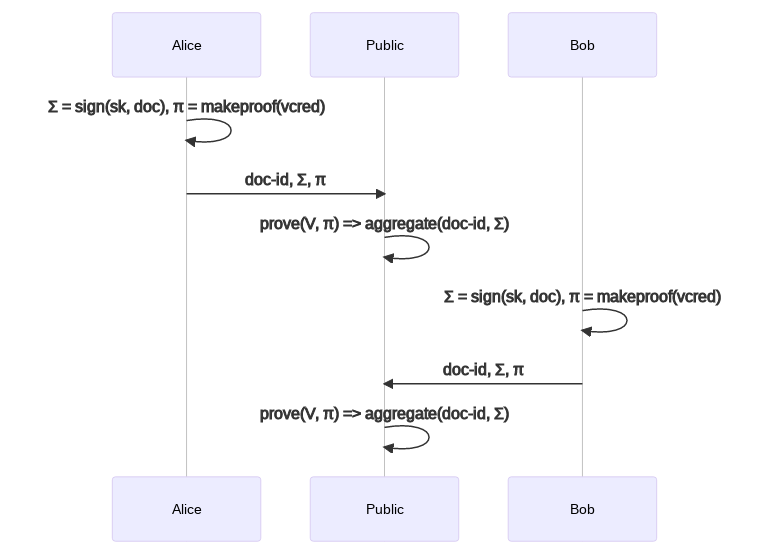
\includegraphics[width=0.4\textwidth]{sign-seq}
\end{figure}

\textbf{Verify:}

\begin{figure}
  \caption{Verification process sequence diagram}
  \centering
  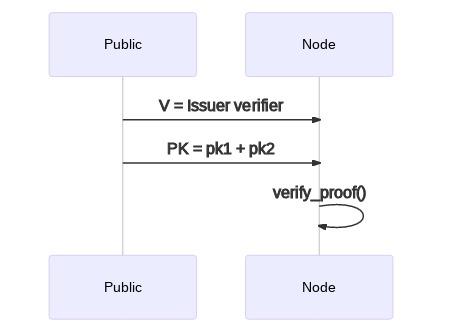
\includegraphics[width=0.4\textwidth]{verify-seq}
\end{figure}



\begin{lstlisting}[style=lua]

---------
-- SETUP
---------

G1 = ECP.generator()
G2 = ECP2.generator()

-- credentials
ZK = require_once('crypto_abc')
issuer = ZK.issuer_keygen()

-- keygen
sk1 = INT.random() -- signing key
ck1 = INT.random() -- credential key
PK1 = G2 * sk1     -- signature verifier

sk2 = INT.random()
ck2 = INT.random()
PK2 = G2 * sk2

-- issuer sign ZK credentials
Lambda1 = ZK.prepare_blind_sign(ck1*G1, ck1) -- credential request:       p -> i
SigmaTilde1 = ZK.blind_sign(issuer.sign, Lambda1)    -- issuer signs credential:  i -> p
Sigma1 = ZK.aggregate_creds(ck1, {SigmaTilde1})  -- credential sigma          p -> store

Lambda2 = ZK.prepare_blind_sign(ck2*G1, ck2)
SigmaTilde2 = ZK.blind_sign(issuer.sign, Lambda2)
Sigma2 = ZK.aggregate_creds(ck2, {SigmaTilde2})

-- sign

UID = ECP.hashtopoint(msg) -- the message's hash is the unique identifier

--------------
-- SETUP done
--------------

print "--------------------------"
print "first base signing session"
r = INT.random()
R = UID * r      -- session

-- add public keys to public session key
PM = (G2 * r) + PK1 + PK2

-- Session opener broadcasts:
-- 1. R   - base G1 point for signature session
-- 2. PM  - base G2 point for public multi-signature key
-- 3. msg - the message to be signed

-- proofs of valid signature
-- uses public session key as UID
Proof1,z1 = ZK.prove_cred_uid(issuer.verify, Sigma1, ck1, UID)
Proof2,z2 = ZK.prove_cred_uid(issuer.verify, Sigma2, ck2, UID)
-- each signer signs
S1 = UID * sk1
S2 = UID * sk2

-- generate the signature
-- each signer will communicate: UID * sk
SM = R + S1 + S2


-- print signature contents to screen
I.print({pub = PM, -- session public keys
		 sign = SM,
		 uid = UID,
		 proofhash1 = sha256( ZEN.serialize( Proof1 ) ),
		 proofhash2 = sha256( ZEN.serialize( Proof2 ) ),
		 zeta1 = z1,
		 zeta2 = z2,
		 issuer = issuer.verify
})

-- verify
assert( ZK.verify_cred_uid(issuer.verify, Proof1, z1, UID),
		"first proof verification fails")
assert( ZK.verify_cred_uid(issuer.verify, Proof2, z2, UID),
		"second proof verification fails")
assert( ECP2.miller(PM, UID)
		   == ECP2.miller(G2, SM),
        "Signature doesn't validates")

\end{lstlisting}

\section{Evaluation}
\label{sec:evaluation}

\lipsum[5]

\bibliographystyle{unsrtnat}

\bibliography{references}

\listoffigures

% \subsection{}
% Citations use \verb+natbib+. The documentation may be found at
% \begin{center}
% 	\url{http://mirrors.ctan.org/macros/latex/contrib/natbib/natnotes.pdf}
% \end{center}

% Here is an example usage of the two main commands (\verb+citet+ and \verb+citep+): Some people thought a thing \citep{kour2014real, hadash2018estimate} but other people thought something else \citep{kour2014fast}. Many people have speculated that if we knew exactly why \citet{kour2014fast} thought this\dots

% \subsection{Figures}
% \lipsum[10]
% See Figure \ref{fig:fig1}. Here is how you add footnotes. \footnote{Sample of the first footnote.}
% \lipsum[11]

% \begin{figure}
% 	\centering
% 	\fbox{\rule[-.5cm]{4cm}{4cm} \rule[-.5cm]{4cm}{0cm}}
% 	\caption{Sample figure caption.}
% 	\label{fig:fig1}
% \end{figure}

% \subsection{Tables}
% See awesome Table~\ref{tab:table}.

% The documentation for \verb+booktabs+ (`Publication quality tables in LaTeX') is available from:
% \begin{center}
% 	\url{https://www.ctan.org/pkg/booktabs}
% \end{center}


% \begin{table}
% 	\caption{Sample table title}
% 	\centering
% 	\begin{tabular}{lll}
% 		\toprule
% 		\multicolumn{2}{c}{Part}                   \\
% 		\cmidrule(r){1-2}
% 		Name     & Description     & Size ($\mu$m) \\
% 		\midrule
% 		Dendrite & Input terminal  & $\sim$100     \\
% 		Axon     & Output terminal & $\sim$10      \\
% 		Soma     & Cell body       & up to $10^6$  \\
% 		\bottomrule
% 	\end{tabular}
% 	\label{tab:table}
% \end{table}



\end{document}
